% This section is dedicated to algorithm which are used in all spectroscopic modes

%-----------------------------------------------------------------------------------------
\subsection{Telluric absorption correction / absolute flux calibration}\label{ssec:tellcorr}
Due to the dense molecular absorptions arising from the Earth's atmosphere, nearly every \ac{MIR} regime spectrum requires a correction for these telluric features. The required atmospheric transmission curve can be achieved either by specific observations of a \ac{TSS} (the "classical" way) or by a modelling approach, e.g. \texttt{molecfit}.\\
As default mode for the telluric correction \texttt{molecfit} is foreseen for all modes. For the \ac{IFU} we assume no major issues, especially as in highly resolved spectra individual line shapes can be fit very well. However, it is to be tested during commissioning, how well that approach works in case of the \ac{LSS} modes, as only blends of lines are visible in the low-resolution regime. We therefore include also the well-proven classical method by means of a standard star.\\
In the \ac{MIR} regime it is possible to use a standard star for both, the telluric correction and the absolute flux calibration, i.e. the conversion of \ac{ADU}s to physical units. This is done by comparing the observed spectrum of a standard star with its reference spectrum as seen without atmospheric and instrument/telescope signatures, facilitating the response function to be determined. This function describes the throughput of the optical system, i.e. the instrumental effect on the flux. In principle this is a standard procedure based on the comparison of an observed spectrum of a spectro-photometric standard star with its flux calibrated model, hence a good model containing intrinsic spectral features as well as absolute fluxes of the individual star is required.\\
Having such observations at hand, telluric correction and flux calibration can be applied simultaneously as one correction function containing the absolute flux and atmospheric absorptions can be derived, if the standard star is observed directly before/after the science target at the same airmass (ideally in the same direction) assuming the atmosphere has not changed significantly in the meantime. The current calibration plan foresees observations of up to two standard stars for \ac{OB}s requiring accurate flux calibration (cf.~\cite{METIS-calibration_plan}, Section 3.8). In that case, this star can be used for the combined purpose. As we do not differ between standard stars for telluric correction and absolute flux calibration refer only to "Standard Stars" (STD) hereafter.\\
For the time being we assume the same (wavelength-dependent) slit-losses in the science and the calibrator observations, i.e. the \ac{AO} performance being stable.  \\

%------------------------------------------------------------------------------
\subsubsection{Classic approach with a standard star}\label{sssec:tecllcorrclassic}
A \ac{STD} spectrum is taken ideally directly before/after the science observations near the science target position (or at least at the same airmass) to probe the same pathway through the Earth's atmosphere. The most simplest approach can be described by
\begin{equation}
    F_\textrm{sci}=F_{0,\textrm{cal}}\cdot\left(S_\textrm{sci}/S_\textrm{cal}\right)\cdot\left(T_\textrm{SkyCalc\_cal} / T_\textrm{SkyCalc\_sci}\right)
\end{equation}
where $S_\textrm{sci}$ and $S_\textrm{cal}$ are the measured fluxes (e.g. in [\ac{ADU}]) of the science target and the standard star and $F_{0,\textrm{cal}}$ is a model of the standard star in physical flux units. Thus, the standard star is used for the flux calibration, i.e. the conversion between \ac{ADU} and physical units to correct for the total instrumental throughput and the sky transparency. In case there's only a marginal difference in airmass between the science and the calibrator target, the airmass compensation can be achieved with synthetic model spectra of the transmission of the science target $T_\textrm{SkyCalc\_sci}$ and the calibrator $T_\textrm{SkyCalc\_cal}$, e.g. with the tool \texttt{SkyCalc}\footnote{\url{https://www.eso.org/observing/etc/bin/gen/form?INS.MODE=swspectr+INS.NAME=SKYCALC}}. Also the latest version of \texttt{molecfit} incorporates a routine for the compensation of airmass differences. This approach should be sufficient even for the \ac{LSS} mode as the wide wavelength range and the low resolving power does not allow to resolve individual telluric lines anyway. The high-resolution mode (\ac{IFU}) enables one to much better determine telluric features and is therefore less prone to problems arising with \texttt{molecfit}.\\
%For the \ac{IFU} mode a more sophisticated approach could be considered: This \ac{STD}-spectrum is processed in the same way as the science spectrum (except the absolute flux calibration). To remove intrinsic stellar features this spectrum is corrected with a model spectrum of this \ac{STD}. Finally its continuum is normalised to unity. The resulting normalised spectrum (ideally) only contains the fingerprint of the Earth's atmospheric absorptions and can be used for the telluric correction.\\
There are several sources for standard spectra available (cf. also Section 4 in~\cite{METIS-calibration_plan}):
\begin{itemize}
    \item Cohen set (\cite{coh99}): Set of 422 stellar model templates, mainly K and M giants. One of the standard sets in \ac{MIR}.
    \item The SPEX \ac{IRTF} Spectral library\footnote{\url{http://irtfweb.ifa.hawaii.edu/~spex/IRTF_Spectral_Library/}}: Set of observed stellar spectra (F to M-type, some carbon and S-type stars and L and T dwarfs) in the range $0.8...5.0\mu$m mostly at a resolving power of $R\equiv\lambda/\Delta\lambda\sim2,000$.
    \item Phoenix library\footnote{\url{https://phoenix.astro.physik.uni-goettingen.de/}}\cite{phoenix}: Library of synthetic medium and high resolution spectra between $0.5...5.5\mu$m covering a wide stellar parameter space ($2,300\textrm{K}\leq T_\textrm{eff}\leq12,000\textrm{K}$; $0.0\leq\log g\leq+6.0$; $-4.0\leq$[Fe/H]$\leq+1.0$; $0.2\leq$[$\alpha$/Fe]$\leq+1.2$).
    \item Flux calibration programme of the \ac{JWST} (\cite{gor22})
    \item "van der Bliek" standards (\cite{vdb96}): 253 L and M band standards
    \item Standard star database from \texttt{CalSpec}\footnote{\url{http://www.stsci.edu/hst/observatory/crds/calspec.html}}: flux standards for the \ac{HST} system (\cite{boh14})
    \item L-band fluxes from 55 near-IR standards from the MSSSO system~\cite{mcg94}
    \item Standards stars from CRIRES\footnote{\url{https://www.eso.org/sci/facilities/paranal/instruments/crires/tools.html}} containing high-resolution spectrophotometric observations of 23 stars (L-band)
    \item  UKIRT standard stars\footnote{\url{http://www.ukirt.hawaii.edu/astronomy/calib/phot cal/}}
\end{itemize}
The \ac{METIS} consortium will soon look into that topic and to assemble a set of appropriate \ac{STD} stars for each observing mode.

%------------------------------------------------------------------------------
\subsubsection{Modelling synthetic transmission spectra}
In the last years the modelling method for the telluric correction has evolved. It is based on radiative transfer modelling of the Earth's atmosphere. A height model of the Earth's atmosphere containing information of pressure, temperature and the concentration of molecules in combination with a radiative transfer model and a molecular line list is used to calculate a transmission function of the Earth's atmosphere at the time of observations. By fitting specific atmospheric absorption features in the science spectra and varying the input height profile allows to determine the state of the Earth's atmosphere at the time of observation. The best-fit transmission function is finally used for the telluric correction.\\
In the past years the approach of modelling transmission curves of Earth's atmosphere has made significant progress leading to versatile and mature software packages for the telluric correction. One of these packages is \texttt{molecfit}\footnote{\url{http://www.eso.org/sci/software/pipelines/skytools/molecfit}} (\cite{mf1, mf2, molecfit}). This software is optimised for the ESO framework and ESO instruments and is also foreseen to be used for \ac{METIS}.\\
The outcome of the \ac{ELT} working group meeting of 2021-03-15 was that future instrument pipelines should include dedicated recipes based on the telluric correction \texttt{telluriccorr} library~\cite{telluriccorr}. This package is based on \texttt{molecfit} and will be provided and maintained by \ac{ESO}. The telluric correction will be performed in three dedicated recipes as post-correction   and closely follow the approach as implemented in the \ac{KMOS} pipeline. The three steps comprise the fit of the telluric features (e.g. \REC{metis_LM_lss_mf_model} for the LM range), the calculation of the transmission curve (e.g. \REC{metis_LM_lss_mf_calctrans}) and the application of the actual correction (e.g. \REC{metis_LM_lss_mf_correct}). The IFU recipe \REC{metis_ifu_telluric} comprises all three steps. For the determination of the \ac{LSF} we primarily rely on the possibilities as offered by the \texttt{telluricorr}/\texttt{molecfit} package, which is based on a fitting of the \ac{LSF} by a combination of a boxcar, Gaussian or Lorentzian. On basis of the commissioning data we will establish a parameter set providing a good starting point for the fits.\\
We also intend to enable the user to include a dedicated line kernel instead, in case a reliable kernel model can be determined with other (external) tools (e.g. a model-based convolution of an internal \ac{LSF}, the slit-widths and/or an \ac{AO} component). In addition, also external supplementary meteorological data (e.g. line-of-sight profiles of water vapour measured by an \ac{LHATPRO} radiometer) can be included if the \texttt{telluricorr}/\texttt{molecfit} and/or \texttt{skycorr} package offers that possibility. 
%------------------------------------------------------------------------------
\begin{figure}[ht]
  \centering
  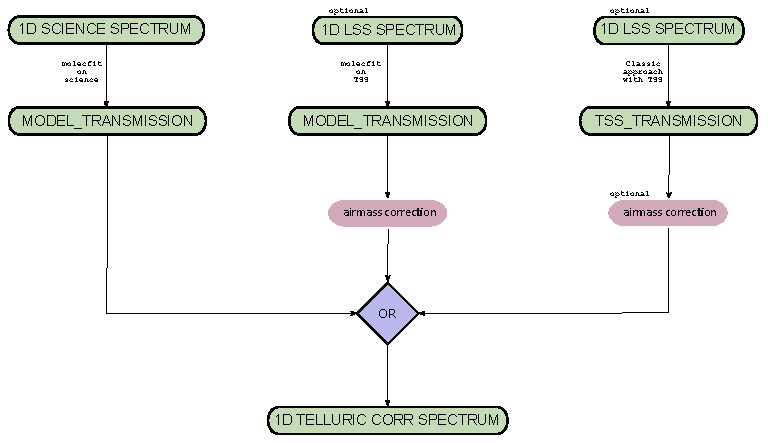
\includegraphics[width=0.9\textwidth]{figures/tell_corr_methods.pdf}
    \caption[Methods for the telluric correction to be included in the METIS pipeline]{%
        Methods for the telluric correction to be included in the \ac{METIS} pipeline.}
  \label{Fig:tellcorrmethods}
\end{figure}
\subsubsection{Approach for METIS}
The modelling approach has become the standard way for the telluric correction in several ESO pipelines as it avoids to spend valuable observing time on taking \ac{STD} spectra. Since the synthetic transmission function is noise-free, it also conserves the \ac{SNR} of the science spectrum. It is therefore  foreseen as default method for the \ac{METIS} pipeline.\\
However, there might be situations where the classical way becomes the better option. For example, in case the science object's continuum is too weak to be used for fitting telluric absorption features and not enough sky emission is available, or the low-resolution \ac{LSS} spectra do not allow to find a good fitting solution due to line blends. In addition, \texttt{molecfit} relies on a number of fitting parameters, which might not lead to the best minimum. In particular, the quality of the fit is very sensitive to the incorporated \ac{LSF}-Kernel, whereas the \ac{LSF} of a \ac{STD} spectrum is naturally (almost) identical.\\
We therefore will include three different approaches for the telluric correction in the \ac{METIS} pipeline (cf. Fig.~\ref{Fig:tellcorrmethods}):
\begin{itemize}
    \item "\textit{molecfit-on-science}": This is the usual way of using \texttt{molecfit}, i.e. the science spectrum ("\texttt{1D SCIENCE SPECTRUM}") is used to determine the state of the Earth's atmosphere and to calculate a synthetic transmission (left branch in Fig.~\ref{Fig:tellcorrmethods})
    \item "classical" approach: The transmission of the Earth's atmosphere is determined in the classical way with the help of a \ac{STD} as described above (right branch in Fig.~\ref{Fig:tellcorrmethods}). In this case, a combined absolute flux calibration / telleuric correction is applied.
    \item "\textit{molecfit-on-star}": This is a combination of the both methods in the sense that \texttt{molecfit} is applied to \ac{STD} observations, and the resulting synthetic transmission spectrum is used for the telluric correction of the science target  (middle branch in Fig.~\ref{Fig:tellcorrmethods})
\end{itemize}
\textit{Additional remarks:}\\
Following the development within the \ac{ELT} working group "Telluric Correction", the newest release\footnote{\url{https://www.eso.org/sci/software/pipelines/}} of \texttt{molecfit} will contain some new features, which will be used in the \ac{METIS} pipelines: (a) a routine to correct transmission spectra for airmass. This allows the usage of \ac{STD} which are at a different airmass than the science target; (b) a method to quantitatively estimate the quality of the telluric correction on the science frames, which will be used for \ac{QC}; (c) a routine to use the wavelength fit as wavelength calibration for the science observations, i.e. to use telluric features as reference frame. For more details on that new features we refer to the \texttt{molecfit} documentation of the upcoming release and the documents in the working group\footnote{\url{https://eso.org/wiki/pub/ELTScience/Telluric_correction/TelluricWG_20230425.pdf}}.\\
As mentioned above, \texttt{molecfit} will be the default method. It is therefore the users sole responsibility to decide whether a \ac{STD} is required/desired. However, the selection of the \ac{STD} should not be arbitrary, but only possible from a provided catalogue.\\
Please note that the workflow in the recipes processing the \ac{STD} stars (e.g. \REC{metis_LM_lss_std}, \REC{metis_N_lss_std} or \REC{metis_ifu_reduce}) changes when the classical method is chosen. In the \texttt{molecfit} case, a telluric correction is applied to the \ac{STD} spectrum to better determine the response function and only the response is delivered to the science recipes. In case of the classical approach, the response function will also contain the telluric features of the \ac{STD}, and therefore a telluric correction beforehand is counterproductive.\\
For the \ac{LSS} mode of \ac{METIS} we intend to implement the flux calibration approach as described in the \ac{HDRL} wherever possible (cf.~\cite{hdrl-manual}).\\ %This method incorporates an automatic telluric correction of the standard star, which can be disabled. This might be useful in case the user decided to observe a dedicated \ac{STD}. 
One of the most critical steps in the framework of \texttt{molecfit} is the fit of the \ac{LSF}. In order to get a first estimate we simulated \ac{LSS} observations of a point source with a constant (i.e. flat) spectrum with ScopeSIM\footnote{\url{https://scopesim.readthedocs.io/en/stable/}\newline\url{https://github.com/AstarVienna/ScopeSim}} in a way to purely get spectra with an unaffected \ac{LSF}. The extracted, background-removed 1d-spectra were used as input for \texttt{molecfit v1.5.9} (see Fig.~\ref{Fig:lss_sim}). We focused on the M and N bands using the fitting regions and molecules given in Fig.~\ref{Fig:lss_sim}. The fitting results in Fig.~\ref{Fig:lss_results} show good coincidence between the input spectra and the fits leading to a fairly good telluric correction (cf. Fig.~\ref{Fig:lss_corr}. 
\begin{figure}[ht]
  \centering
  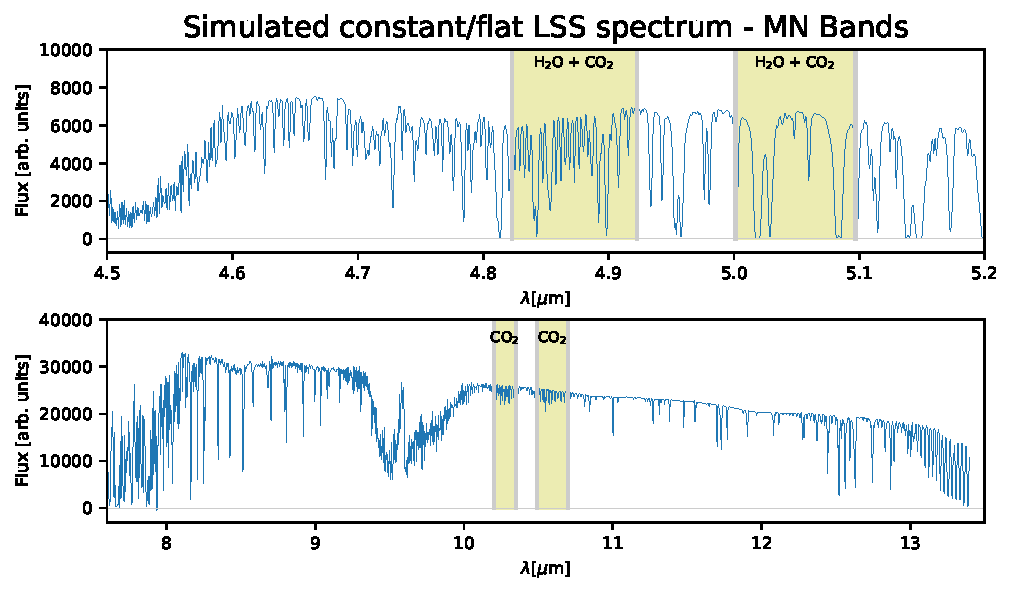
\includegraphics[width=1.0\textwidth]{figures/LSS_CrtAlg_files/LSS_sim_spectra.pdf}
    \caption[Simulated spectra of a flat source with telluric absorptions]{%
        Simulated 1D LMN-Band spectra of a flat source with telluric absorptions. The yellow shaded areas show the fitting regions of the incorporated molecules (M-band: H$_2$O and CO$_2$ between 4.82 and 4.92$\mu$m and 5.0, 5.1$\mu$m; N-band: CO$_2$ between 10.2, 10.35$\mu$m and 10.49, 10.7$\mu$m}
  \label{Fig:lss_sim}
\end{figure}
\begin{figure}[ht]
  \centering
  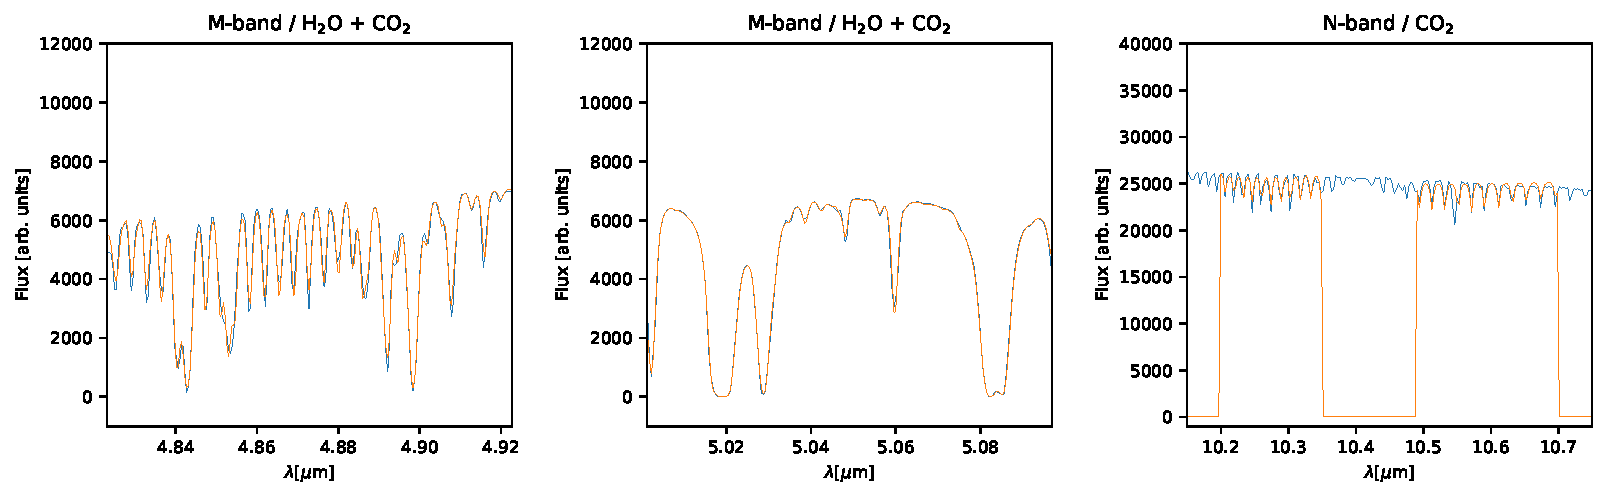
\includegraphics[width=1.0\textwidth]{figures/LSS_CrtAlg_files/LSS_mf_details.pdf}
    \caption[Molecfit details]{%
        Telluric corrections of the \ac{LSS} M and N-band spectra in the selected regions; green: resulting transmission, blue: uncorrected spectrum; orange: corrected flux}
  \label{Fig:lss_results}
\end{figure}
\begin{figure}[ht]
  \centering
  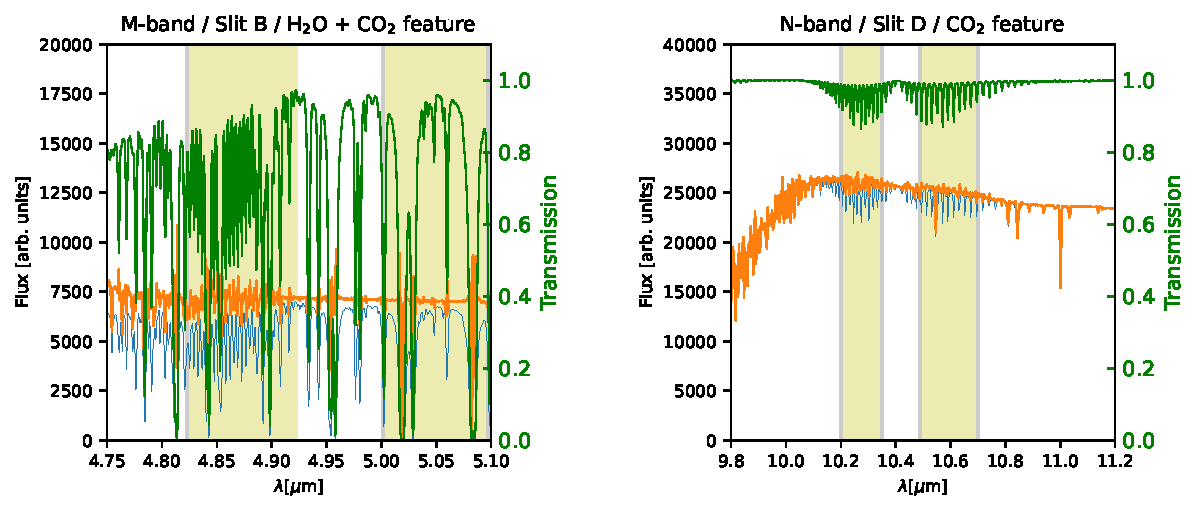
\includegraphics[width=1.0\textwidth]{figures/LSS_CrtAlg_files/LSS_mf_results.pdf}
    \caption[Molecfit results]{%
        Fitting results with \texttt{molecfit 1.5.7}: The blue curve shows the input spectrum, the orange curve is the fit
  \label{Fig:lss_corr}
\end{figure}

%------------------------------------------------------------------------------
%\subsubsection{Other algorithms included in the telluric correction approach}\label{ssec:otheralgstellcorr}
\subsubsection{Quality control parameters for \texttt{molecfit}}\label{ssec:tellcorr_qc_params}
%\paragraph{Normalisation of \ac{STD} continua\newline}\label{ssec:spec_normalisation}
%The normalisation of spectra can be a tricky issue especially for cool stars with plenty intrinsic spectral features. A general approach is therefore not possible. However, we can restrict our routines to stars, which are (a) well-known and (b) model spectra are available. We therefore use the following approach: 
%\begin{itemize}
%    \item For each star we determine spectral regions, which are known to belong to the continuum, i.e. do not contain absorption/emission features, neither intrinsic nor atmospheric.
%    \item These spectral regions are then fit by a polynomial (or alternatively the Rayleigh-Jeans approximation is used). The degree of the polynomial will be determined when the set of \ac{STD} is established. 
%    \item The \ac{STD} spectrum is finally divided by this polynomial leading to a spectrum normalised to unity.
%\end{itemize} 

%\paragraph{Airmass correction of transmission functions\newline}\label{ssec:airmass_corr}
%As mentioned above
%\begin{equation}
%    \left(T_\textrm{SkyCalc\_cal} / T_\textrm{SkyCalc\_sci}\right)
%\end{equation}

%\paragraph{Quality control parameters for \texttt{molecfit}\newline}\label{ssec_tellcorr_qc_params}
To estimate the quality of the telluric correction we follow the approach incorporated with the new \texttt{molecfit} version 4.3.1:
\begin{itemize}
    \item Smoothing the corrected spectrum with a Savitzky-Golay filter\footnote{\url{https://en.wikipedia.org/wiki/Savitzky\%E2\%80\%93Golay_filter}}
    \item dividing the corrected spectrum by the smoothed one; This leads to a normalisation to unity and a crude removal of slopes and intrinsic features
    \item Determine the mean absolute difference of the resulting spectrum, excluding \texttt{NaN} values on the user provided spectral ranges (e.g., only spectral ranges with telluric features). 
\end{itemize}
